 \section{Partial Suppression Algorithm}
\label{sec:algo}

%\renewcommand{\algorithmicforall}{\textbf{for each}}
%\algnotext{ENDFOR}
%\algnotext{ENDIF}
%\algnotext{ENDWHILE}

The Optimal Suppression Problem defined in Section \nameref{sec:prob} is
an NP-hard problem\cite{meyerson2004complexity}.
%To find the optimal suppressor,
%the naive approach needs to try suppressing all combinations of items,
%with a complexity of $O(2^N)$ where $N$ is the total number of items in $T$.
We therefore present the partial suppression algorithm as a
heuristic solution to the Optimal Suppression Problem.
%By definition of a safe set-valued table (Definition
%\ref{def:safety_table}), the breach probability of each \qid in $Q$ must be
%under the threshold $\rho$ (Definition \ref{def:safety_qid}).
%For
%example, given a \qid $q=\{a, b, \alpha\}$ and all its linked sensitive items
%$\linked(q)=\{\beta\}$, where $\{a, b\}$ are non-sensitive items and
%$\{\alpha, \beta\}$ are sensitive items, if $\csize(q)=5$, $\csize(q \cup
%\{\beta\})=3$ and $\rho=\frac{1}{3}$, then $\breach(q)=\frac{3}{5}>\rho$.
%\begin{definition}[Data Structures]
%We define three key data structures in this framework.
%$B$ is a \qid buffer which is a set of \qids.
%$K$ is a mapping which is essentially a materialized function from \qid $q$ to $\csize(q)$.
%$L$ is a mapping from \qid $q$ to $\linked(q)$.
%\end{definition}
To simplify the discussion of the algorithm, we make the following
definitions.
%
%\textcolor{green}{ Do we need this?
%\begin{definition}[Data Structures]
%We define three key data structures in this framework. $B$ is a \qid buffer
%which stores a set of \qids. $S$ is a \textbf{mapping} which is essentially a
%materialized function from \qid $q$ to $sup(q)$. $L$ is a \textbf{mapping}
%from \qid $q$ to $\linked(q)$.
%\end{definition}
%In the following algorithms, we will also use $sup(\cdot)$ and
%$\linked(\cdot)$ to denote the computations of these two functions, and use
%$S(\cdot)$ and $L(\cdot)$ to denote the access of the elements of the two
%data structures.
%}
%\KZ{This whole thing is not clear, need to rephrase:
\begin{lemma}
\label{minimum}
%Number of suppressions is defined as the number of items that must be
%deleted to disable an unsafe sensitive association rule.
To disable an unsafe rule $q \rightarrow e$, the minimum number of instances
of item type $t \in q\cup\{e\}$ (denoted as $N_s(t, q\rightarrow e)$) 
that needs to be suppressed is
\begin{equation}\label{eq:N_s}N_s(t, q\rightarrow e)=
\begin{cases}
\max(0, sup_T(q\cup \{e\})-sup_T(q)\rho) & t=e  \\
\max(0, \frac{sup_T(q\cup \{e\})-sup_T(q)\rho}{1-\rho}) & t\in q %\\
% \infty & otherwise
\end{cases}
\end{equation}
\end{lemma}
\begin{proof}
Suppose we suppress $X$ items, where $X$ is the largest number such that
$X<N_s(t, q\rightarrow e)$.\\
If $t = e$,
\begin{eqnarray*}
conf(q \to e)&=&\frac{{{{\sup }_{T'}}(q \cup \{ e\} )}}{{{{\sup }_{T'}}(q)}}\\
&=&\frac{{{{\sup }_T}(q \cup \{ e\} ) - X}}{{{{\sup }_T}(q)}}\\
&>&\frac{{{{\sup }_T}(q \cup \{ e\} ) - {N_s}(t,q \to e)}}{{{{\sup }_T}(q)}}\\
&=&\frac{{{{\sup }_T}(q \cup \{ e\} ) - ({{\sup }_T}(q \cup \{ e\} ) - {{\sup }_T}(q)\rho )}}{{{{\sup }_T}(q)}}\\
&=&\rho
\end{eqnarray*}
If $t\in q$,
\begin{eqnarray*}
conf(q \to e)&=&\frac{{{{\sup }_{T'}}(q \cup \{ e\} )}}{{{{\sup }_{T'}}(q)}}\\
&=&\frac{{{{\sup }_T}(q \cup \{ e\} ) - X}}{{{{\sup }_T}(q) - X}}\\
&>&\frac{{{{\sup }_T}(q \cup \{ e\} ) - {N_s}(t,q \to e)}}{{{{\sup }_T}(q) - {N_s}(t,q \to e)}}\\
&=&\frac{{{{\sup }_T}(q \cup \{ e\} ) - \frac{{{{\sup }_T}(q \cup \{ e\} ) - {{\sup }_T}(q)\rho }}{{1 - \rho }}}}{{{{\sup }_T}(q) - \frac{{{{\sup }_T}(q \cup \{ e\} ) - {{\sup }_T}(q)\rho }}{{1 - \rho }}}}\\
&=& \rho
\end{eqnarray*}
In both of these cases, the confidence of the unsafe rule is still larger than $\rho$.
 So the data is not sufficiently suppressed. Therefore $N_s(t, q\rightarrow e)$ is the minimum number of suppressions to make $q \rightarrow e$ safe.
%\qed
\end{proof}

%Of all item types in $q\cup e$, there exists an item type $t_{min} \in q\cup
%e$ which results in minimum suppressions.
In other words, we need to delete at least $N_s(t, r)$ instances of item $t$ to make it safe. We select these instances randomly for deletion.
\newtheorem{Definition}{Definition}

\begin{Definition}[Leftover]
 The leftover of item type $t$ is defined as
 % \vspace{-1mm}
\begin{equation}
leftover(t)={sup_{T'}(\{t\})}/{sup_T(\{t\})}
\end{equation}
\end{Definition}
$T$ is the original data and $T'$ is the intermediate suppressing result.
The ratio shows the percentage of remaining instances of item $t$
in the intermediate result $T'$.
%More items suppressed indicates a smaller ratio.


%\XJ{move this para to algo sec} \MakeRed{
The key intuition of our algorithm is that even though the total number of
``bad'' sensitive association rules is exponential in the worst case, 
incremental ``invalidation'' through partial suppression 
%of a small number of affected items 
can massively reduce the number of these bad rules, 
which leads to quick convergence.
% to a solution.
%}
%%%
%
%In this paper, we adopts three kinds of partial suppression policies.
%The first one is \PartialR, which suppresses only sensitive items
%in the consequents. The second one is \PartialL, which
%suppresses only items in the antecedents.
%The third one is \PartialALL, which suppresses items in
%both the consequents and the antecedents.
%\PartialL and \PartialALL suppress both sensitive
%and non-sensitive items, whereas \PartialR suppresses only
%sensitive items.
%Next we present the basic algorithm of this framework.

\subsection{The Basic Algorithm}
\label{sec:basic}

%To ensure a table is safe, we must make sure all \qids in $Q$ are safe.
\PartialSuppression~ (Algorithm \ref{algo:partialsuppression}) presents the
top-level algorithm. The partial suppressor iterates over the table $T$, and
for each record $T[i]$, the algorithm first generates  \qids from $T[i]$ and
sanitizes the unsafe ones. The suppressor terminates when the whole table is
scanned and there is no unsafe \qid.

% \vspace{-6mm}
%\newtheorem{algorithm}{algorithm}

\begin{algorithm2e}[h]
\small
\caption{$\PartialSuppression(T,\bmax)$}
\label{algo:partialsuppression}
\begin{algorithmic}[1]
   % \STATE Initialize $safe\leftarrow\TRUE$, $i\leftarrow 1$;
  %  \STATE Initialize $safe\leftarrow\TRUE$
\STATE Shuffle $T$ (original table)
\STATE $T_0 \gets T$ %(original table)
\STATE $i\leftarrow 1$
\STATE $safe \leftarrow \TRUE$
    \LOOP
        \STATE Clear buffer $B$
        %\STATE {Initialize the $sup$ of all \qids to 0}
        \WHILE {$|B|<b_{max}$ \AND $i\leq |T|$} \label{algo:enu_s}
            \STATE $qids \gets$ \qids generated from $T[i]$
	    \IF {$|qids|>b_{max}$}
		\STATE \textbf{exit}
            \ELSIF {$|B \cup qids|>b_{max}$}
                \STATE \textbf{break}
            \ELSE
	     \STATE Update $sup$ of \qids \label{algo:enumerate2}
             \STATE Merge $qids$ into $B$ \label{algo:enumerate1}
             \STATE $i\leftarrow i+1$
            \ENDIF
        \ENDWHILE \label{algo:enu_e}
		%\STATE \textcolor{red}{update $sup$, $\linked$, $S$, $L$;}
%        \STATE Calculate $\rho$ of each $qid$ in $|B|$ \label{algo:update}
%        \IF {$B$ contains an unsafe \qid}\label{line:containunsafe}
        \STATE $safe \leftarrow \SanitizeBuffer(T_0, T, B, H)$\label{line:sanitizebuffer}
%            \STATE $safe\leftarrow\FALSE$
%        \ENDIF
        \IF {$i \ge |T|$} %\AND $safe$}
            \IF {$safe$}
                \STATE \textbf{break}\label{algo:partialbreak}
            \ELSE
                \STATE $i\leftarrow 1$
                \STATE $safe\leftarrow\TRUE$
%                \STATE \textbf{continue}
            \ENDIF
        \ENDIF
    \ENDLOOP
\end{algorithmic}
\end{algorithm2e}

% \vspace{-6mm}
A \qid is a combination of different items,
and the number of distinct \qids to be enumerated is exponential.
We therefore introduce a fixed size \qid buffer of
capacity $\bmax$ to trade space for time of qid generation.
The value of $\bmax$ is significant. Small $\bmax$ values cause
repetitive generation of \qids, while large $\bmax$ values cause the generation
of useless \qids, which do not exist in the data
by the time they are to be processed in the queue. 
%Note that if $\bmax$ is too small to hold the \qids generated from one
%record, the algorithm exits with an exception.
$H$ denotes a heuristic function to be explained 
in the next section.

\subsection{Buffer Sanitization}
\label{sec:sanitize}
Each time \qid buffer $B$ is ready, \SanitizeBuffer
(Algorithm \ref{algo:sanitize}) is invoked to start processing \qids in $B$
and make all of them safe. $D_S(T)$ denotes the domain of all sensitive
items in $T$.
%We first partition \qids in $B$ into two groups, {\em safe} and {\em unsafe}.
%according to Definition \ref{def:probability} and
%\ref{def:safety_qid}.
In each iteration (Lines \ref{algo:pick_rs}-\ref{algo:pick_re}),
\SanitizeBuffer first picks an unsafe $qid$ from $B$,
 and identifies the ``best'' unsafe sensitive association rule
%whose confidence is above $\rho$
to sanitize, according to a user-defined heuristic metric function $H$
implementing a corresponding suppression policy.
Although any heuristic function maybe supplied here, 
we implemented distinct strategies, namely
$H_{dist}$ that preserves the data distribution and $H_{mine}$ that preserves
useful association rules. 
$P$ is a temporary $qid$ buffer that stores the those unsafe $qid$s that 
have been processed.
%Next we discuss the two heuristics.

% \vspace{-6mm}
\begin{algorithm2e}
\caption{$\SanitizeBuffer(T_0, T, B, H)$}
\label{algo:sanitize}
\begin{algorithmic}[1]
%\STATE $\policy \leftarrow \SuppressionPolicy()$ \label{choose_heur}
\STATE $safe \leftarrow \TRUE$
\WHILE{there is an unsafe \qid $q$ in $B$}\label{algo:pick_rs}
    \STATE $safe \leftarrow \FALSE$
    \STATE $E \gets \{e ~|~ conf(q \rightarrow e) > \rho \land  e \in D_S(T)\}$
    %\IF {$\policy = Distribution$}
        %\STATE $(d, q, e) \gets\underset{d\in q\cup E, q, e \in E}{\arg\max}\,H_{dist}(d, q, e, T_0, T)$
        %\STATE {\textcolor{red}{$(d, e) \gets\underset{d\in q\cup E, q, e \in E}{\arg\max}\,H_{dist}(d, q, e, T_0, T)$}}
        \STATE $(d, e) \gets\underset{d\in q\cup E, e \in E}{\arg\min}\, H(d, q, e, T_0, T)$
        \label{algo:heur_dist}
    %\ELSIF {$\policy = Mine$}
        %\STATE $(d, q, e) \gets\underset{d\in q\cup E, q, e \in E}{\arg\min}\,H_{mine}(d, q, e)$
        %\STATE {\textcolor{red}{$(d, e) \gets\underset{d\in q\cup E, q, e \in E}{\arg\min}\,H_{mine}(d, q, e)$}}
        %\STATE {\textcolor{red}{$(d, e) \gets\underset{d\in q\cup E, q, e \in E}{\arg\min}\,MetricFunction()$}}
        %\label{algo:heur_mine}
    %\ENDIF
%    \IF {$\policy = Distribution$}
%        \STATE  find $\SA(q,e)$ with maximal $H_{dist}(d)$, where
%        \STATE  $d\in q\cup\{e\}$ \AND $conf(q,e)>\rho$
%        \label{algo:heur_dist}
%    \ELSE
%        \STATE find $\SA(q,e)$ with minimal $H_{mine}(d)$, where
%        \STATE  $d\in q\cup\{e\}$ \AND $conf(q,e)>\rho$
%        \label{algo:heur_mine}
%    \ENDIF
    \STATE $X\leftarrow q\cup\{e\}$
    \STATE $k\leftarrow N_s(d,q \rightarrow e)$\label{line:sanitize-k}
    \STATE $P\leftarrow \emptyset$
    \WHILE{$k>0$}\label{line:sanitize-whilek}
        \STATE randomly pick a record $R$ from $T$ where
		$R\subseteq \container(X)$ \label{pick_row}
        \STATE Add \qids containing $d$ in $R$ to $P$
        \STATE $R\leftarrow R-\{d\}$\label{line:sanitize-suppress}
        \STATE $k \leftarrow k-1$
    \ENDWHILE
    \STATE Update $sup$ of \qids in $P$ \label{algo:update_kl}
\ENDWHILE \label{algo:pick_re}
\STATE \textbf{return} $safe$
\end{algorithmic}
\end{algorithm2e}

%% \vspace{-6mm}
%\begin{algorithm}
%\caption{$\SuppressionPolicy()$}
%\label{algo:metricFunc}
%\begin{algorithmic}[1]
%    \STATE \textcolor{red}{$\policy \leftarrow the suppression policy adopted$}
%    \IF {\textcolor{red}{$\policy = Distribution$}}
%
%        \RETURN {\textcolor{red}{$H_{dist}(d, q, e, T_0, T)$}}
%    \ELSIF {\textcolor{red}{$\policy = Mine$}}
%
%        \RETURN {\textcolor{red}{$H_{mine}(d, q, e)$}}
%    \ENDIF
%\end{algorithmic}
%\end{algorithm}

\subsubsection{Preservation of Data Distribution}
%We first present the heuristic function which helps to preserve data
%distribution.
Consider an unsafe sensitive association rule $q \rightarrow e$ where
$conf(q \rightarrow e) > \rho$, and $q \in B$.
%$q$ is thus not a safe by Definition \ref{def:safety_qid}.
To reduce $conf(q,e)$ below $\rho$,
%we must make the confidence
%of the inference not larger than $\rho$, thus
we suppress a number of instances of item $t\in q \cup \{e\}$ from
$\container(q\cup \{e\})$.\footnote{We define $\container(X)=\{T[i]|X\subseteq T[i], 1\le i\le |T|\}$.} We hope to minimize $KL(T ~||~ T_0)$.

%(see \eqnref{eq:kl}).

%, that is
%the difference in probability distribution between the suppressed table $T$
%and the original table $T_0$.
%$\mathcal{A}(q,e)$ and decide the minimum number of occurrences of $t$ to be
%deleted from  $\mathcal{A}(q,e)$ or just eliminate this inference from $T$.
%Kullback-Leibler divergence is defined as
% \[KL(Q||P)=\sum_{t\in
%D}Q(t)log\frac{Q(t)}{P(t)}\]
%where P(t) is the original distribution of $t$
%and $Q(t)$ is the current
%% (before selecting this removal)
% distribution of $t$, which is often used to characterize the distribution
% distance.

%From \eqnref{eq:kl}, 
By the definition of KL divergence in \tabref{table:notations}, 
suppressing some instances of item $t$
where $T(t)>T_0(t)$ ($T_0$ means the original datset),
%\footnote{We denote the probability of item $t$ in $T$ as $T(t)$, 
%which is computed by $\frac{sup_T(t)}{|T|}$.}
the KL divergence tends to decrease. 
Thus we define the following heuristic function:
\begin{equation}\label{eq:hdist}
H_{dist}(t, q, e, T_0, T) =
	\frac{N_s(t, q\rightarrow e)}{T(t)log\frac{T(t)}{T_0(t)}}.
\end{equation}
%The numerator in \eqnref{eq:hdist} indicates the divergence of
%the data distribution on item $t$ only.
%The larger the absolute value is, the larger distribution difference of
%$t$ now is compared with the original
%situation.
%However, if the value is less than 0, i.e. $T(t)< T_0(t)$, we'd
%better not suppress $t$, since it may further decreases $Q(t)$ and
%deteriorates the data distribution. Therefore the larger the numerator is,
%the item has more priorities to be chosen to suppress.
%The denominator indicates the minimum number of items $t$ that needs
%to be suppressed.
%The smaller the number is, the fewer items are suppressed.
Minimizing this function aims at
suppressing item $t$ which maximally recovers the original
data distribution and minimizes the number of deletions.
%Each time we choose a sensitive association rule and a corresponding item $t$
%with the highest $H_{dist}$ value to sanitize (Line
%\ref{algo:heur_dist} in Algorithm \ref{algo:sanitize}).

%
% By iterating over all unsafe \qids, we can all sensitive
%inferences whose confidence larger than $\rho$ from those {\em unsafe} \qids.
%Then in each iteration, the algorithm fetches one sensitive association
%$\SA(q,e)$ and fix it.

\subsubsection{Preservation of Useful Rules}
%\subsubsection{\textcolor{red}{Reduction of Spurious Rules}}
%Then we introduce our second heuristic function which trys to retain minable
%rules with fewer spurious rules invented.
%As we mentioned before, to learn from the characteristic of global
%suppression (no spurious rules introduced), we devise a heuristic which takes
%deletions towards global suppression while using partial suppression.

A spurious rule ($q \rightarrow e$) is introduced when
the denominator of $conf(q \rightarrow e)$, $sup(q)$,
is sufficiently small so that the confidence becomes large enough.
%In order to reduce the introduction of spurious rules,
%our objective to suppress the item whose suppression will result in the least number of spurious rules.
However, if $sup(q)$ is too small, the rule would not have enough
support and can be ignored.
%\PC{Since we do not publish certain data mining results, we can not
%eliminate spurious rules after anoymization.}
Therefore, our objective is to continue suppressing
those items that have been suppressed before,
to minimize the support of the potential spurious rules.
Hence we propose the objective function:
\begin{equation}\label{eq:hmine}
H_{mine}(t, q, e, T_0, T)=leftover(t)\cdot N_s(t, q\rightarrow e)
\end{equation}
and seek to minimize it.

Since the $leftover(t)$ reflects the extent to which an item type $t$ has been suppressed,
the minimization of the objective function tends to suppress an item type 
that has been heavily suppressed before.
In the meantime, it leaves those less suppressed item types
unaffected and thus protect them from
the potential introduction of spurious rules caused by the suppression.
%\begin{equation}\label{eq:hmine}
%H_{mine}(t, q, e)=N_r(t, q\rightarrow e)\cdot N_s(t, q\rightarrow e)
%\end{equation}
%, where $N_r(t, q\rightarrow e)$ denotes the number of spurious rules the suppression of item $t$ will introduce.
%}
%as a heuristic function which is to be minimized
%in Line \ref{algo:heur_mine} of Algorithm \ref{algo:sanitize}.
%
%$leftover(t)$ represents remaining content of item $t$ and
%$N_s(t, q\rightarrow e)$ represents the minimum number of item
%$t$ that needs to be suppressed to satisfy the privacy model.
%%
%The product expresses
%the strategy that we want to introduce fewer spurious rules by imitating the
%effect of global suppression while suppressing as few items as possible.
%%
%As we can see, each time we choose the sensitive association rule with lowest
%$H_{mine}$ to perform sanitization (Line \ref{algo:heur_mine} in Algorithm \ref{algo:sanitize}).

%However, $H_{mine}$ goes the opposite side of preserving the original data
%distribution. Therefore, we introduce the following heuristic function
%separately to preserve the original data distribution and minimizes the
%deletion in local optimal.
%
%
%\subsubsection{Rest of the Algorithm}
%% Next we will show the two heuristic
%% functions that help to find the `best` association to fix.

\subsubsection{Regression}
After suppressing the item $d$ from a record, 
some unsafe \qids containing $d$ may become safe, while other safe \qids
containing $d$ may become unsafe again.
This is an undesirable situation known as {\em regression}, which, doesn't 
happen with the global suppression.
Line \ref{algo:update_kl} of
Algorithm \SanitizeBuffer determines the set of
\qids that would be affected by regression. This step is like the $qid$
generation step in Algorithm \PartialSuppression~ Line \ref{algo:enumerate2}
and \ref{algo:enumerate1}. There are different ways to pick a
record from $\container(q\cup \{e\})$ to suppress item $d$ (Line
\ref{pick_row}). Our strategy is to pick records randomly from $\container(X)$.
%The deletion of one particular item $d$ affects not only the rules
%related to the $qid$ ${d}$, but also those related to $qid$s that
%contain $d$ and other item types.
Randomly choosing records actually spreads the change of support across 
many different \qids, such that the possibility of a safe \qid becoming unsafe is
reduced. This alleviates the effect of regression.
%can smooth the impact caused by
%the deletion of $d$ on each of the other item types,
%and thus avoid introducing spurious rules.
\cut{%%%%%%%%%%%%%%%%%%%%%% begin of cut %%%%%%%%%%%%%
\begin{table*}[th]
\caption{A Running Example}
\centering
%\subtable[The Original Dataset]{
%\begin{tabular}{|c|l|}
%\hline
%% after \\: \hline or \cline{col1-col2} \cline{col3-col4} ...
%{\bf TID} & {\bf Transaction} \\ \hline
%1 & bread, milk, {\em condom} \\ \hline
%2 & bread, milk  \\ \hline
%3& flour, fruits  \\ \hline
%4& flour, {\em condom}\\ \hline
%5& bread, fruits  \\ \hline
%6& fruits, {\em condom}  \\ \hline
%\end{tabular}
%\label{tab:sample1}
%}
\subtable[Step 1 for $H_{mine}$]{
\begin{tabular}{|c|l|}
\hline
% after \\: \hline or \cline{col1-col2} \cline{col3-col4} ...
{\bf TID} & {\bf Transaction} \\ \hline
1 & bread, milk, {\em condom} \\ \hline
2 & bread, milk  \\ \hline
3 & milk, {\em condom}  \\ \hline
4& flour, fruits  \\ \hline
5& flour, \sout{{\em condom}}\\ \hline
6& bread, fruits  \\ \hline
7& fruits, {\em condom}  \\ \hline
\end{tabular}
\label{tab:sampledata2}
}
\subtable[Step 2 by $H_{mine}$]{
\begin{tabular}{|c|l|}
\hline
% after \\: \hline or \cline{col1-col2} \cline{col3-col4} ...
{\bf TID} & {\bf Transaction} \\ \hline
1 & bread, milk, \sout{{\em condom}} \\ \hline
2 & bread, milk  \\ \hline
3 & milk, {\em condom}  \\ \hline
4&flour, fruits  \\ \hline
5& flour, \sout{{\em condom}}\\ \hline
6& bread, fruits  \\ \hline
7& fruits, {\em condom}  \\ \hline
\end{tabular}
\label{tab:sampledata3}
}
\subtable[Step 1 by $H_{dist}$]{
\begin{tabular}{|c|l|}
\hline
% after \\: \hline or \cline{col1-col2} \cline{col3-col4} ...
{\bf TID} & {\bf Transaction} \\ \hline
1 & bread, milk, {\em condom} \\ \hline
2 & bread, milk  \\ \hline
3 & milk, {\em condom}  \\ \hline
4& flour, fruits  \\ \hline
5& \sout{flour},{\em condom}\\ \hline
6& bread, fruits  \\ \hline
7& fruits, {\em condom}  \\ \hline
\end{tabular}
\label{tab:sampledata4}
}
\subtable[Step 2 by $H_{dist}$]{
\begin{tabular}{|c|l|}
\hline
% after \\: \hline or \cline{col1-col2} \cline{col3-col4} ...
{\bf TID} & {\bf Transaction} \\ \hline
1 & bread, milk, \sout{{\em condom}} \\ \hline
2 & bread, milk  \\ \hline
3 & milk, {\em condom}  \\ \hline
4&flour, fruits  \\ \hline
5& \sout{flour}, {\em condom} \\ \hline
6& bread, fruits  \\ \hline
7& fruits, {\em condom}  \\ \hline
\end{tabular}
\label{tab:sampledata5}
}
\end{table*}
}%%%%%%%%%%%%%%% end of cut %%%%%%%%%%%
%\subsubsection{Data Distribution or Rule Mining?}
%The two heuristic functions aim at different downstream applications.
%%We argue that the user can choose the corresponding heuristic with regard
%%to their specific demands.
%$H_{dist}$ typically causes suppressions of different types of items whereas
%$H_{mine}$ tends to focus on deleting one type of items. This is evident
%from the results shown in Table \ref{tab:sample3} and Table \ref{tab:sample4}.
%%one type of item in the whole dataset in that the latter one will remove all those $bad~rules$
%%containing this item.
%Furthermore, to preserve data distribution, usually more items need to be
%suppressed than to preserve useful association rules.
%%Furthermore, less items will normally represent less association rules.
%This type of trade-off between data distribution and rule mining inspires
%our design of the two heuristic functions.
%

\cut{%%%%%%%%%%%%%%% begin of cut %%%%%%%%%%%%
\subsubsection{A Running Example}
\label{sec:appendix}

\begin{table}
\caption{Sensitive Rules in the Running Example}
\centering
\subtable[Sensitive Rules Table 1]{
\begin{tabular}{|c|c|c|c|}
\hline
% after \\: \hline or \cline{col1-col2} \cline{col3-col4} ...
TID & \qid &Sensitive Item & $\rho$ \\ \hline
1   &  bread, milk& {\em condom}&  1/2\\ \hline
2& bread &{\em condom}& 1/3\\ \hline
3& milk& {\em condom}& 2/3 \\ \hline
4&flour& {\em condom} &1/2 \\ \hline
5&fruits&  {\em condom} &1/3 \\ \hline
\end{tabular}
\label{tab:sampleRule1}
}
\subtable[Sensitive Rules Table2 ]{
\begin{tabular}{|c|c|c|c|}
\hline
% after \\: \hline or \cline{col1-col2} \cline{col3-col4} ...
TID & \qid &Sensitive Item & $\rho$ \\ \hline
1   &  bread, milk& {\em condom}&  1/2\\ \hline
2& bread &{\em condom}& 1/3\\ \hline
3& milk& {\em condom}& 2/3 \\ \hline
4&fruits&  {\em condom} &1/3 \\ \hline
\end{tabular}
\label{tab:sampleRule2}
}
\end{table}


In this section, we demonstrate how our algorithm works step-by-step
using the example data set in Table \ref{tab:sample}.
We assume $\rho=1/3$ in this privacy model and ``condom'' is a sensitive item,
while all other items are non-sensitive.

The original dataset is given in Table \ref{tab:orig-sample}.
Assume that all the \qids could be stored in the buffer and we show each step in the buffer sanitization process.
The original sensitive rules are shown in table \ref{tab:sampleRule1}.

We first show how to suppress the table for rule mining using $H_{mine}$.
Rule 1, rule 3 and rule 4 all have the smallest $H_{mine}$ with $N_s(condom, q\rightarrow condom)$ =1 and $leftover(condom)$=1 in table \ref{tab:sampleRule1}. Then we randomly pick one rule from these three rules. We pick rule 4
in table \ref{tab:sampleRule1} as our candidate and
sanitize this rule by deleting ``flour'' or ``condom'' once to satisfy our privacy model. We choose to delete ``condom'' in this example, but the program may choose ``flour''
since the information loss is the same.
After this step, Table \ref{tab:orig-sample} turns into
Table \ref{tab:sampledata2} and the sensitive rules are updated in
Table \ref{tab:sampleRule2}. In Table \ref{tab:sampledata2},
``condom'' in rule 1 and rule 3 have the least $H_{mine}$ with
the value $\frac{3}{4}$ in that $leftover(condom)$=$\frac{3}{4}$ and
$N_s(condom, q\rightarrow condom)=1$. Therefore, we choose to
sanitize rule 1 by eliminating ``condom''.
Eventually, we get a safe table in Table \ref{tab:sampledata3}.

Next we choose $H_{dist}$ as our heuristic function.
Notice that all sensitive rules in Table  \ref{tab:sampleRule1}
have the same $H_{dist}$ with the value 0 since the
distribution of the data is not altered before suppression.
Therefore, we pick the rule with the smallest
 $N_s(t, q\rightarrow t)$. Suppose we choose rule 4 as our candidate and
delete ``flour'', then the original table turns into
Table \ref{tab:sampledata4} and sensitive rules
table also becomes Table \ref{tab:sampleRule2}.
In Table \ref{tab:sampledata4}, ``condom'' in rule 1 and rule 3 has
 the highest $H_{dist}$ 0.006 (see table \ref{tab:sampleRule2}). Then we delete ``condom'' in transaction 1 and get a safe table \ref{tab:sampledata5}.
}%%%%%%%%%%%%%%%%%%%%%%end of cut %%%%%%%%%%%
%
%\subsection{\textcolor{red}{Speed-up of $sup$ Update}}
%\textcolor{red}{The immense scale of transaction data calls for a well-designed method to store and update the $sup$ of \qids.
%If upon every update of the $sup$, we go through the whole transaction table to count the presence of a specific \qid,
%the process will be time-consuming.
%In this work, we adopt a $trie$ structure to store the $sup$s.}
%
%\textcolor{red}{Every node on the $trie$ represents an item type.
%The items contained in all transactions are pre-sorted in a special order.
%For simplicity, here we assume that the item types are denoted by English letters $A,B,C...$
%and the items in a transaction are ordered alphabetically.
%An attribute is attached to every node
%which records the number of transactions whose first several items are exactly the ones on the path from the root to the very node.
%For example, as shown in Fig.\ref{fig:trie}, there is a letter and a number at each node.
%The letters are item types and the numbers are the values of the attributes.
%The value of the attribute of the root node $A$ is 11.
%It means that there are 11 transactions that begin with item type $A$.
%}
%
%\begin{figure}[tb]
%\centering
%%\subfigure[Example of the Trie Structure]{
%\hspace{-1cm}
%\begin{minipage}[c]{0.45\textwidth}
%\centering
%  \includegraphics[width=7cm]{trie.eps}
%\end{minipage}%
%%}
%\caption{Example of the $Trie$ Structure}\label{fig:trie}
%\end{figure}
%
%\textcolor{red}{
%When the $sup$ of a \qid is queried, the program will quickly find the related \qids on the $trie$
%and calculate the $sup$. For example, if the $sup$ of \qid $\{F\}$ is queried,
%since \qid $\{F\}$ appears in the transactions that begin with $\{A,B,F\}$, $\{A,C,F\}$ and $\{A,F\}$,
%the result of $2+1+2$ will be returned.}
%

\subsection{Optimization with Divide-and-Conquer}
\label{algo:impmentation}

When the dataset is very large we can speed up by
a divide-and-conquer (DnC) framework that
partitions the input data dynamically,
runs \PartialSuppression~
on them individually and combines the results in the end. This approach is
correct in the sense that if each suppressed partition is safe. 
%(this will be shown in Section \ref{sec:eval}).

\begin{algorithm2e}
%\caption{Top level partitioning controller}
\caption{$\SplitData(T,\tmax)$} \label{algo:splitdata}
\begin{algorithmic}[1]
    \IF { $Cost(T) > \tmax$ }
        \STATE Split $T$ equally into $T_1$ , $T_2$
        \STATE $\SplitData(T_1,  \tmax)$
        \STATE $\SplitData(T_2, \tmax)$
    \ELSE
        \STATE $\PartialSuppression(T,  \bmax)$
    \ENDIF
\end{algorithmic}
\end{algorithm2e}

Algorithm \ref{algo:splitdata}
splits the input table whenever the estimated cost of
suppressing that table is greater than $\tmax$.
Here $\tmax$ is the maximum execution time allowed.
Whenever the estimated cost of suppression the data exceeds
$\tmax$, the data is split into two equal portions.
%For simplicity we randomly partition the original data in two
%\footnote{Recall that the input table is a set of records with
%no predefined order} when the estimated time is above $\tmax$.
Cost is estimated as:
\begin{equation}\label{eq:costfunc}
Cost(T)=\frac{|T| \cdot 2^\frac{N}{|T|}}{|D(T)|} 
\end{equation}
%where $\mathcal{AVG}$ is the average transaction size, i.e. $\frac{N}{|T|}$,
where $N$ is the total numbers of items in $T$. 
The function estimates the average number of qids per item type. 
%The larger this value is, the more sensitive association rules
%we may need to handle.
%This estimate of $Cost(T)$ is derived in more detailed 
%next in \secref{sec:imp}.

In order to guarantee the consistency in data distribution between the 
original problem and the sub-problems, when splitting $T$ equally 
into $T_1$ and $T_2$, we randomly assign half of the items in 
$T$ to $T_1$ and the remaining items to $T_2$ .
%The function estimates the
%average number of \qids per item type. The larger this value is, the more
%sensitive association rules we should handle. The cost function is used when
%data size is large enough. We argue that when $|T|$ is relatively
%small there is no need to apply DnC.

\subsection{Analysis of the Algorithm}
\label{sec:analysis}

% Analyze the main algo: time complexity, space complexity.
% Some properties to consider:
%
% \begin{itemize}
% \item give a bound on the total number of items suppressed;
% \item give a bound on the deviation in distribution from the original data;
% \item give a bound on the number of association rules that we eliminate;
% \item and what else??
% \end{itemize}
We present some theoretical results along with their proofs
in order to provide a comprehensive view of the problem and our algorithm.

\subsubsection{Correctness}
\begin{lemma}%[Correctness of partitioning]
\label{CorrectnessOfPartitioning}
  If $q$ is safe in both $T_1$ and $T_2$, then $q$ is safe in $T = T_1 \cup T_2$.
\end{lemma}
\begin{proof}
For any item $a$,
  \begin{align*}
   q~\text{is safe in}~T_1 &\Rightarrow sup_{T_1}(q\cup\{a\}) \le \rho\cdot sup_{T_1}(q) \\
   q~\text{is safe in}~T_2 &\Rightarrow sup_{T_2}(q\cup\{a\}) \le \rho\cdot sup_{T_2}(q)
  \end{align*}
  So \begin{align*}
   sup_{T_1}(q\cup\{a\}) + sup_{T_2}(q\cup\{a\}) &\le \rho\cdot sup_{T_1}(q) + \rho\cdot sup_{T_2}(q)
  \end{align*}
  Furthermore,
  \begin{align*}
    sup_T(q\cup\{a\}) &= sup_{T_1}(q\cup\{a\}) + sup_{T_2}(q\cup\{a\}) \\
    sup_T(q) &= sup_{T_1}(q) + sup_{T_2}(q)
  \end{align*}
  Therefore, $$ \frac{sup_T(q\cup\{a\})}{sup_T(q)} \le \rho~\Rightarrow q~\text{is safe in}~T.$$ 
\end{proof}

\newtheorem{Theorem}{Theorem}

\begin{Theorem}
\label{CorrectnessOfPartialSuppression}
  \PartialSuppression~ always terminates with a correct solution.
\end{Theorem}
\begin{proof}
We first prove that if the algorithm terminates, the suppressed table is safe.
Note that the algorithm can only terminate on Line \ref{algo:partialbreak}
  in Algorithm \ref{algo:partialsuppression}.
  Therefore, two conditions must be satisfied. First, the record cursor
$i$ should exceed the table size $|T|$. Second, the value $Safe$ must be \TRUE.
$Safe$ is true iff there is no unsafe \qids in the table, otherwise  Line \ref{algo:sanitize}
 will assign $Safe$ to \FALSE. If $i$ exceeds $|T|$ and
$Safe$ is \TRUE, the algorithm
must have scanned the table at least once and
hasn't found any unsafe \qids. 
%Hence, the suppressed table is safe.

Then we prove that \PartialSuppression~ always terminates by measuring the
  number of items left (denoted $l$) in the table after each step of suppression.
Initially, \[l=l_0=\sum_{i=1}^{|T|} |T[i]|\le |D(T)| |T|.\]
We state that for every invocation of \SanitizeBuffer that returns false, 
Line \ref{line:sanitize-suppress} in Algorithm \ref{algo:sanitize} is 
executed at least once.
If this is the case, then the value $l$ strictly decreases by a positive integer
whenever \SanitizeBuffer returns false. Since $l$ is originally finite,
the algorithm will terminate unless \SanitizeBuffer always return true.
If \SanitizeBuffer keep returning true, after the whole table is passed,
the algorithm also terminates.
%Otherwise there will be an infinite descending chain of all the $l$ values.

Now we prove that Line \ref{line:sanitize-suppress} in Algorithm \ref{algo:sanitize}
  is executed at least once whenever \SanitizeBuffer returns false.
%Whenever \SanitizeBuffer is invoked, it is guaranteed that there exists
%  an unsafe \qid $q\in B$ (see Line \ref{line:containunsafe}  in Algorithm \ref{algo:partialsuppression}).
$q$ is unsafe so that there always exists an item $e\in\linked(q)$ such that $conf(q,e)>\rho$,
  i.e. \[ \frac{sup(q\cup\{e\})}{sup(q)}>\rho \Rightarrow
   sup(q\cup\{e\})-\rho\cdot sup(q)>0 .\]
For $k$ on Line \ref{line:sanitize-k} in Algorithm \ref{algo:sanitize},
  \[ k = N_s(t, q\rightarrow e)\]
  and
  \[N_s(t, q\rightarrow e) \geq sup(q\cup\{e\})-\lfloor\rho\cdot sup(q)\rfloor \ge 1\]
  as shown in Lemma \ref{minimum}. Therefore,
  it is guaranteed that the number of deletions is at least 1, 
  because the rule $q\rightarrow e$ is unsafe and there must be some deletions to make it safe.
So $k\ge 1$ on Line \ref{line:sanitize-whilek} for the first time.
Thus the condition is satisfied and Line \ref{line:sanitize-suppress} is executed.
%\qed
\end{proof}

\newtheorem{Corollary}{Corollary}

\begin{Corollary}
The divide-and-conquer optimization \SplitData~ is correct.
\end{Corollary}
\begin{proof}
It follows directly from Lemma \ref{CorrectnessOfPartitioning} and
Theorem \ref{CorrectnessOfPartialSuppression}. %\qed
\end{proof}

\subsubsection{Overall Time Complexity}
\label{sec:imp}
%\textcolor{red}{In this section, we will discuss the implementation of the algorithms and analyze the time complexity.}
We analyze the time complexity of Algorithm \ref{algo:partialsuppression}.
%Before the execution of \PartialSuppressor, \SplitData~
%splits the data set into smaller parts.
%This phase takes negligible time and is ignored in the analysis.
In each iteration, there are two phrases of computation. First (phase 1), the while loop which generate $qid$s and populate the buffer $B$. Second (phase 2), 
the \SanitizeBuffer function is called to make sure every 
unsafe $qid$s in $B$ becomes safe by suppressing a number of items from $T$.

Because the number of generated $qid$s is very large, phase 1 is bounded by the size of the buffer $b_{max}$. Update of the $sup$ of a $qid$ takes constant time due to the use of a hash map. Therefore, phase 1 takes $O(b_{max})$ time.

Phase 2, has an outer while loop which
loops at most $b_{max}$ times, that is when all $qid$s in $B$ are unsafe. 
Inside the outer while loop, the most expensive steps are Line \ref{algo:heur_dist} and the inner while loop. 
Line \ref{algo:heur_dist} needs to enumerate different combination of $d$ and $e$. 
The total number of combinations is $N/|T|\times(1-\rho)|D_S(T)|$,
where size of $q \cup E$ is bounded by the average length of a record in $T$,
and the size of $E$ is bounded by $(1-\rho)|D_S(T)|$. The inner while loop
is bounded by $k$, which is the number of suppressions made. 
Thus the phase 2 costs $O(b_{max} (N/|T|\times(1-\rho)|D_S(T)| + k))$.

We can estimate the number of iterations as $N/k$, 
thus the overall complexity is
\[O\left(b_{max}\frac{N}{k} +b_{max}(\frac{ N(1-\rho)|D_S(T)|}{|T|}+ k)
\frac{N}{k}\right).\]
Finally, as shown in the proof of Theorem \ref{CorrectnessOfPartialSuppression},
$k$ is strictly greater than zero. In the worse case, we can estimate the number of 
iterations in  Algorithm \ref{algo:partialsuppression} by $N$, that is, when
$k=1$ and all items in $T$ are suppressed. The overall time complexity
is thus simplified to:
\begin{equation}
O\left(\frac{b_{max} N^2(1-\rho)|D_S(T)|}{|T|}\right). \label{eq:timecomp}
\end{equation}

%\KZ{Below is the old version...}
%We use a hashmap to store all the distinct $qid$s generated as well as their corresponding $sup$s.
%In addition, a linked map is created for each distinct $qid$,
%which stores the sensitive item types that co-occurs with the $qid$ in a transaction record $T[i]$
%and the number of co-occurrences.
%To calculate all the values in the hashmap and the linked map,
%we need to generate every possible $qid$ from all the transaction records.
%As such, $2^{|T[i]|}$ $qid$s can be generated from one record $T[i]$.
%For convenience, the average length of record $\frac{N}{|T|}$ is used instead of $|T[i]|$ in the calculation.
%
%We need to pick an unsafe $qid$ before sanitizing the buffer.
%Therefore we have to calculate the $conf(q,e)$ for each $qid$ generated and their linked sensitive items.
%Here $q$ refers to a $qid$ and $e$ refers to a sensitive item contained in $q$'s 
%linked map. Let $M$ be the maximum size of any linked map.
%$conf(q,e)$ will calculated at most $M$ times for any $qid$.
%
%Both heuristic functions require to scan all the unsafe $qid$s,
%whose size is at most $b_{max}$. Then the heuristic function value for each
%$(q, e)$ pair is calculated and the most suitable item type $d$
%is chosen for suppression. $d$ will be randomly deleted from
%transaction records where $q$ and $d$ co-occur.
%The linked maps save a lot of time in finding
%records containing both $q$ and $d$. However, the maximum time consumed
%is still bounded by $|T|$.
%%In the process of deleting items, some operations are  $|T[i]|$ (the length of each record) times, such as finding the items exactly equal to our goal item $d$ in \SanitizeBuffer Algorithm.
%%They don't cost much comparing to the operations above.
%
%Finally, since $M$ is smaller than $|T|$, the time complexity for 
%each iteration is bounded by 
%\begin{equation}\label{eq:complexity}
%O(2^{\frac{N}{|T|}}\cdot |T|+b_{max}\cdot M +b_{max}\cdot |T|) = O((2^{\frac{N}{|T|}}+b_{max})\cdot |T|).
%\end{equation}
%Can we bound the number of iterations??
%Notice that the analysis is conservative.
%In fact, the search for most $qid$s and items takes less time than above,
%because items are usually distributed in only some of the records, but not all of them.
%Since the most time consuming component of the algorithm is generating and
%finding the $qid$s, we choose to estimate the cost of suppressing a dataset $Cost(T)$
%by $|T|\cdot 2^{\frac{N}{|T|}}$, i.e. the first term in \eqref{eq:complexity}.
%
